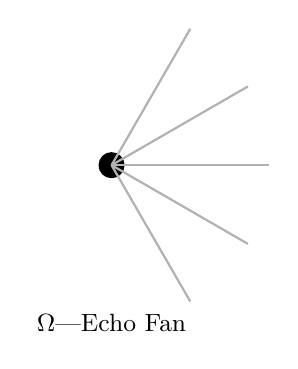
\begin{tikzpicture}[
    arc/.style={thick, draw=gray!60},
    node/.style={circle,fill=black,minimum size=5pt}
]

\node[node] at (0,0) {};

\foreach \a in {-60,-30,0,30,60}{
    \draw[arc] (0,0) -- ++({2*cos(\a)},{2*sin(\a)});
}

\node at (0,-2) {\small $\Omega$---Echo Fan};

\end{tikzpicture}